\documentclass[11pt]{article}
%Gummi|065|=)
\usepackage{graphicx}
\usepackage{tikz}
\usepackage{amsmath}
\usepackage{listings}
\usepackage{textcomp}


\lstset{
  language=bash,
  basicstyle=\ttfamily
}
\graphicspath{ {./images/} }
\title{\textbf{Rank\textbf{}ing of Graphs Simulation}}
\author{Janith Perera\\[1cm]{\small Advisor: Prof. Zsolt Tuza}}
\date{03/05/2019}
\begin{document}

\maketitle
\pagebreak
\tableofcontents
\listoffigures
\pagebreak
\section{Introduction}

In this paper, it describes the implementation of the simulation software \big(\textbf{graph\_simulacra}) which ranks the tree graphs. The general idea behind the software is to provide a platform to simulate the graphs, and rank the vertices based on the hierachy and degree. The software is build upon a programatical algorithm to find the vertex ranking, which is a solution proposed to the optimal vertex ranking. \\*

\noindent
The current implementation of the platform is a prototype and it is a desktop application, which natively supports for \textbf{UNIX} platforms. It has very basic usecase to operate, however, it mainly target on the algorithm, and generating the graph and saving as an image. 




\section{Functional Overview}

The graph\_simulacra contains two user operations, which are \textbf{add} and \textbf{save}. In \textbf{add} operation, it prompts a file browser to choose the input text file and once the graph is generated, the image can be saved in a similar method by using \textbf{save} operation. 

\begin{figure}[ht]
\centering
     
\includegraphics[width=1.0\textwidth]{Diagram1.png}
      \caption{Basic operations flow chart}
       \label{normal_case}
\end{figure}

\noindent
The file extension of the intput file is not restricted, how ever, it is recommend to use \textbf{.txt} extension for the input file, as it has to be a plain text file. The output image file will be formatted as png, which will be explained in a later section.

\subsection{Input Subroutine}

The input subroutine accepts only \textbf{adjecency matrix} to generate the graph. In graph theory, \textbf{adjecency matrix} is a square \big($n\times$n) matrix which represents finte graphs. The eliments of the matrix shows the adjecency for each vertices and hence it is a \big(0,1) matrix, 1 is used to show the adjecency between respective nodes. 

\[
   M=
  \left[ {\begin{array}{ccccc}
   0 & 1 & 0 & 0 & 0 \\
   1 & 0 & 1 & 0 & 0 \\
   0 & 1 & 0 & 1 & 0 \\
   0 & 0 & 1 & 0 & 1 \\
   0 & 0 & 0 & 1 & 0 \\
  \end{array} } \right]
\]

\vspace{5mm}

\noindent
The above adjecency matrix is  $5\times5$ matrix, which belongs to very basic line graph. It has five nodes and two leaves.\\ 

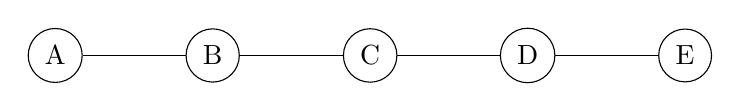
\begin{tikzpicture}

    \node[shape=circle,draw=black] (A) at (0,4) {A};
    \node[shape=circle,draw=black] (B) at (2,4) {B};
    \node[shape=circle,draw=black] (C) at (4,4) {C};
    \node[shape=circle,draw=black] (D) at (6,4) {D};
    \node[shape=circle,draw=black] (E) at (8,4) {E};

   \draw[-,black]   (A) -- (B);
   \draw[-,black]   (B) -- (C);
   \draw[-,black]   (C) -- (D);
   \draw[-,black]   (D) -- (E);
\end{tikzpicture}

\subsubsection{File Format}

The input file should provide the adjecency matrix to the program. However, to represent the matrix, the format cannot be the same as it showed in the previous section. It maintain the simplicity, it uses a slightly different format, which is still meaningful and easy to follow.\\* 

\noindent
The matrix is construct as comma separated values and new lines. The rule of \big($n\times$n) must be kept as it will not produce a proper graph. \\*

\begingroup
\centering
\verb|0,1,0,0,0|\\*
\verb|1,0,1,0,0|\\*
\verb|0,1,0,1,0|\\*
\verb|0,0,1,0,1|\\*
\verb|0,0,0,1,0|\\*

\endgroup
\vspace{5mm}

\noindent
You may use any text editor to write this file and save as a text file, preferably with \textbf{.txt} extension.
Once you save the file, click on \textbf{Add} button and select the file to load as a graph. \\


\subsection{Interface}

This is a small overview of the user interface and there will be much detailed technical overview in a later section. The user interface is basically a desktop GUI, and it is not a resizable window. 

\begin{figure}[ht]
\centering
     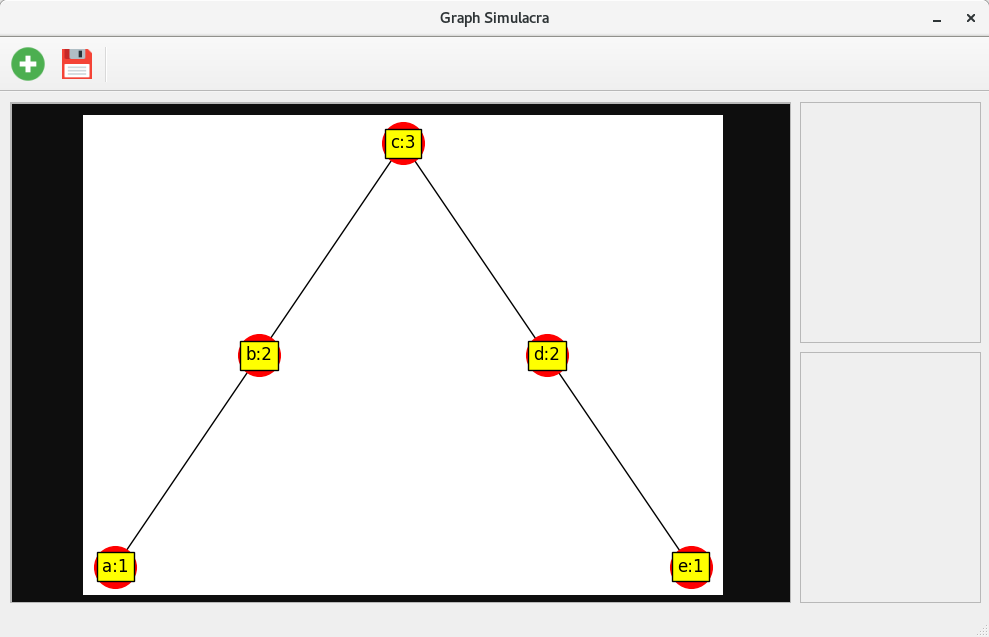
\includegraphics[width=1.0\textwidth]{window.png}
      \caption{Graph Simulacra MainWindow}
       \label{normal_case}
\end{figure}

\subsubsection{Layout}

The top bar consists of two buttons, which are already scribed in the previous section. \textbf{Add} and \textbf{Save} respectively in the top menu icons.\\*

\noindent
The generated graph displays in the center of the window, which is a web view. \\*

\noindent
The left bar shows the information regarding each and every node. From this information tabs, the user can have better understanding of the graph vertices.\\*

\noindent
The entire window will have the same gtk color scheme as it is defined by the host operating system. 

\section{Ranking Algorithm}

This is the main part of the program, where it ranks all the vertices with a proper ranking machinsm. Let's consider the step by step procedure of the ranking. In this task, it uses two subroutines, one is to rank leaves and the other subroutine to rank the rest of the graph. 

\begin{itemize}
  \item Get degree of vertices
  \item Find leaves (degree = 1)
  \item Rank leaves as 1 and set other vertices to 2
  \item Iterate every other (new) vertices, which are not leaves
  \item [iteration]
  \item The neighbours of each vertex must have eiter similar, minor rank or superior rank
  \item If all ranks are minor, then continue
  \item If neighbours equal ranks, increase self rank by 1.
  \item If both equal and minor ranks exist, then increase equal rank neighbour by 1
  \item If superior ranks and equal ranks exist, then increase self rank by max rank + 1 (here it doesn't check about minor ranks)
\end{itemize}
\subsection{Pseudo Python Code}
\begin{lstlisting}[language=Python]
node_list = []
for i in range(len(G)):
    if i not in exclude_nodes:
        nb_dict = []
        self_idx = i
        self_rank = current node rank
        for n_node in list(G.neighbors(i)):
            nb_dict = get node idx and rank

        list_of_nb_ranks = get node rank list

        if max_node < self_rank:
            continue
        elif max_node == self_rank and min_node 
        == self_rank:
            self_node = str(self_rank+1)
        elif max_node == self_rank and min_node 
        < self_rank:
            for i in [get node idx = to self_rank]:
                i node = str(self_rank+1)
        elif max_node > self_rank and self_rank in 
        list_of_nb_ranks:
            self_node = str(max_node+1)
        node_list.append(i)
            
return node_list
\end{lstlisting}
\section{Technical Overview}

\subsection{Development platform}

\textbf{graph\_simulacra} is totally written in Python programing language, and the version is 3.6. It uses several frameworks and other libraries which will be discussed in later sections. The development environment is GNU Linux, which gives great support for Python projects. 

\subsubsection{Packaging}

The packaging of the Python project is achieved by using \textbf{Cookie Cutter} framework, which is popular in generating an ideal file structure to maintain the package. The framework supports for many other popular programing languages, how ever, initially it is originally designed to support Python packaging.

\subsubsection{Prerequisites}

As it mentioned before, there are some requirements must be meet, prior to execution of the program. The Python version plays a critical role, as the backward compatibility is not garanteed. Other requirements are basically the frameworks and libraries which are used in runtime. All the required libraries and respective versions are included in the \textbf{requirements.txt} and use the following method to install them.

\begin{lstlisting}
  pip install -r requirements.txt
\end{lstlisting}

\subsubsection{Repository \& Installation}

The other important part of the development platform is, the code repository. For this project, the code repository is public repository of \textbf{github.com}. Please note the following installation guide.

\begin{itemize}
	\item install git tools to the host machine
	\item Project url
\begin{lstlisting}
  https://github.com/jantwisted/graph_simulacra.git
\end{lstlisting}
	\item Clone the project
\begin{lstlisting}
  git clone <project url>
\end{lstlisting}
	\item Goto the project directory
	\item Install prerequisites
\begin{lstlisting}
  pip install -r requirements.txt
\end{lstlisting}
	\item Install the program
\begin{lstlisting}
  sudo python setup.py install
\end{lstlisting}
	\item Execute the program
\begin{lstlisting}
  graph_simulacra -X
\end{lstlisting}	
\end{itemize}

\subsection{GUI Interface}

The GUI interface is built on Qt framework, which is a cross platform UI interface. As it says in the definition, it supports for almost all the major desktop platforms and most mobile or embedded platforms, including Unix like operating systems. Most GUI programs created with Qt have a native-looking interface, in which case Qt is classified as a widget toolkit.\\* 

\noindent
Qt supports various compilers, including the GCC C++ compiler and the Visual Studio suite and also it has libraries for \textbf{Python} environments. \\*

\noindent
In this project, it uses \textbf{Qt5} and the \textbf{simulacra\_ui.py} file contains the UI interface declaration, which is the main window class. QT Designer is used in creating the interface graphically, which is convinient to have an intensive design. QT Designer produces an xml file, which is the generic way of designing with Qt framework and with combination of \textbf{pyuic} tool and Qt Designer, the UI interface declaration class has been generated.\\*

\noindent
The interface declaration class has a few main Qt components. The components are common in most of the Qt projects. However, web module is not necessory for all GUI programs, however as for a enhancement to the display, it includes web widget as well.

\begin{itemize}
	\item QtWidgets \\
	QtWidgets module provids a set of UI elements to create classic desktop-style user interfaces. These are the primary elements for creating user interfaces in Qt. They can display data and status information, receive user input, and provide a container for other widgets that should be grouped together. 
	\item QWebEngineView \\
	A web view is the main widget component of the Qt web browsing module. It used in displaying the generated graph image in the main window.
	\item Qt Main Window \\
	The Main Window provides a main framework for building the user interface. \textbf{QMainWindow} class is the container for all the other related classes. It has its own layout to add other classes, such as QToolBars, QDockWidgets, QMenuBar and QStatusBar. The layout has a center area that cany kind of widget can be placed. 
\begin{figure}[ht]
\centering
     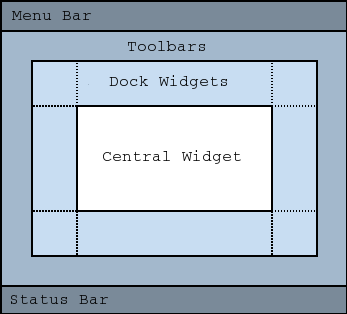
\includegraphics[scale=0.8]{mainwindowlayout.png}
      \caption{Qt MainWindow Layout}
       \label{normal_case}
\end{figure}
\end{itemize}
\pagebreak 
\subsection{NetworkX}

NetworkX is a python library, which used in study of the structure, creation and manipulation of complex networks.It has several mathematical implementations, to simulate graphs which are given by standard and nonstandard data formats. The following list shows some of the related features used in this project.

\begin{itemize}
	\item study the structure and dynamics of the given data set
	\item standard programing interface and graph implementation
	\item an interface to some numerical algorithms
	\item manipulation and combination of other libraries for extensive use
\end{itemize}


\subsection{NumPy}

NumPy is a fundamental package for scientific calculations in Python. However, for this project, it uses only N-dimensional array object data structure. An N-dimensional array\big(ndarray) is a multidimensional container for the items of the same size and type. The shape defines the number of items and the dimensions of the array, which is a tuple of N positive integers. As with other Python data structures like, tuples, lists and dictionaries, the contents of the ndarray can be accessed and modified by indexing or slicing and attributes of the ndarray. The data type supported by an array can be accessed via the 'dtype' attribute on the array. The dimensions of an array can be accessed via the 'shape' attribute that returns a tuple describing the length of each dimension.  In general, ndarray are considered as views to another array, which uses parse of reference method in many implementations. The implementation of adjecency matrix parser which is explained in the below paragraph. \\

\noindent
The ndarray is generated by using a standard Python list, which is fetched from the input file. Once the ndarray Python list is casted to ndarray, it is passed to \textbf{NetworkX} method called \textbf{from\_numpy\_matrix}. From this method, it generates a structural graph, which is only a presented by set of numerical data.\\

\noindent
This implementation shows that \textbf{NetworkX} library support for the other libraries to extend the use of it and also it helps to build much more advanced implementations in fetching data to the Graph object.

\subsection{Matplotlib}
Matplotlib is a Python library to generates 2D plots based on given data set. It produces variety of hardcopy formats and interactive environments across platforms. It mainly used in documentations and reports, however it can be used in anyother Python implementation. Metplotlib has its numerical mathematics extension, which is NumPy, which was explained in the earlier section. The combination of a few libraries with Matplotlib, works similar as MATLAB, and the Python alternative to MATLAB, SciPy also makes use of Matplotlib.

\section{Drawing the Graph}
Let's consider a graph \big(\textbf{G}), when G gets the \textbf{ndarray} data, G \textrightarrow G'. Then G' will be passed to a subroutine to set ranks of each vertices. \\
\begin{lstlisting}[language=Python]
G = nx.from_numpy_matrix(adjacency_matrix)
G = set_ranks(G)
\end{lstlisting} 
\noindent
\\Then G' vertices will be relabled from ASCII alphabet letters respectively for each vertex, along with its relavent rank. Example: \big[\textbf{a:1}]\\
\begin{lstlisting}[language=Python]
G = nx.relabel_nodes(G, labels_map, copy=False)
\end{lstlisting}
\noindent
\\All the similar rank vertices must be horizontally aligned, therefore the node positions must be altered to accordingly. There is a special subroutine to map both nodes and their position and return a dictionary, which will be used in the NetworkX draw layout, along with G'\\
\begin{lstlisting}[language=Python]
fixed_positions = get_fixed_positions(rank_list, 
labels_map)
fixed_nodes = fixed_positions.keys()
plt.figure()
g_nodes = nx.spring_layout(G, pos=fixed_positions,
 fixed = fixed_nodes)
\end{lstlisting} 
\noindent
\\Finally, G' is ready to be plotted and as the project has imported the Matplotlib library, NetworkX library collaborates with it to draw the graph in graphical interface. For further actions, Matplotlib library provides some functionality to the graphic representation of the graph. In this project, it uses Matplotlib function to save the graphical image in a temporary directory for later use.
\begin{lstlisting}[language=Python]
plt.savefig('/tmp/testplot.png')
\end{lstlisting}
\pagebreak
\section{Conclusion}
The applications of ranking graphs can be seen in scheduling problems of assembly steps in manufacturing systems, and \textbf{Graph\_simulacra} is a proposed prototype to simulate such graphs with rankings for given input matrix. The visual presentation of the graph and the arrangment of the vertices position makes the user to get a better overview and also relabeling and rearranging will make user to have less interaction in the process of simulating the graph. As it is a prototype for a bigger software solution, in the long run, the input mechanism, algorithmic optimizations and improved visual presentation with much more interactive way must be considered.


\begin{thebibliography}{999}

\bibitem{ranking}
  H.L. Boldaender, J.S. Deogun, K. Jansen, T. Kloks, D. Kratsch, H. Muller and Zs. Tuza,
  \emph{Rankings of graphs}.
  1995.
\bibitem{optimal}
  Ananth V. IYER, H. Donald RATLIFF, G. VIJAYAN,
  \emph{Optimal Node Rankings Of Trees}.
  1988.
\bibitem{datascience}
  Jake VanderPlas,
  \emph{Python Data Science Handbook}.
  1st Edition, 2016.

\end{thebibliography}
\end{document}

 
